\chapter{软件补丁兼容性检测方法}

本章主要对兼容性问题和其检测方法进行概括介绍。

\section{兼容性问题}
\label {sec_problem}
如前所述,随着软件版本的演进,往往会发生专为某版本设计的补丁无法适用于新版本代码的情况,而如果要为新版本代码重新开发适用的补丁,又耗时耗力极大。因此,本文研究在软件演进背景下,补丁对于其他软件版本的兼容性问题。该问题的主要难点在于如何检测补丁应用于其他软件版本的代码时是否发生冲突。

回顾章节~\ref{sec:background} 中提到的应用场景,某开发团队在其项目中使用了某开源第三方软件,并针对该项目的实际需要对其开发了专门的补丁。现在第三方软件进行了版本升级,该团队需要知道,如果在项目中集成该新版本,原补丁是否还能适用。
%\begin{itemize}
%	\item 
%	\item 
%\end{itemize}

考虑到版本更新也可以使用补丁来完成,该问题就可以从另一种角度来看待,即在集成该新版本的时候,检测原补丁是否能够继续使用的过程可以转化为检测原补丁是否会和升级补丁产生冲突的过程。也就是说,软件补丁对于其他版本的适用性可以从补丁之间的冲突这一角度来考虑。

由于每个补丁都可以视作一系列的变更集合,其中的每条变更都会修改原有代码版本的语法结构,并可能会对其他语法结构造成语义上的影响,那么从这一角度来看时,补丁的兼容性检测问题就得到了简化。如果能够找到每个补丁中的变更所影响到的程序语法结构的集合,那么通过判断这两个集合之间是否存在着一定的交集就能够确定补丁间的语义影响是否会相互覆盖。

显然,如果两个补丁中的变更影响到了相同的语法结构,由于该位置上的语法结构受到了双重影响,该位置就可能出现冲突。这是由于该位置上的语法结构受到了双重影响,而这些影响之间可能存在冲突,无法共存。例如对某条件判断语句而言,原补丁在某处对其引用的变量值进行了修改,使得条件语句中该值增加,而升级补丁中在另外一处对该变量的修改则会导致条件语句中其值减少,显然,这样的双重影响是矛盾的。

当然,在某些情况下,这样的双重影响也是可以共存的。例如上文条件判断语句的例子中,如果两个补丁中的修改都会导致该条件语句中引用的某变量值增加,那么这样的双重影响就可能是兼容的。

这类双重影响并没有严格的规则来判断是否一定冲突或不冲突,因此,只能通过人工分析来辅助判断。

综上所述,软件补丁的兼容性检测问题可以归结为多次变更之间的冲突检测问题。

\section{检测方法概述}
\label {sec_method}

根据上文的讨论,本文提出了一种软件补丁兼容性的检测方法,该方法的整体流程可以参考图~\ref{all_flow}。该方法分为三步。首先,将软件补丁应用于其他版本的代码上,并防止该过程中引入语法错误。其次,找到补丁中的变更所影响到的其他语法结构,也就是后文中提到的变更影响域。最后,根据找到的变更影响域进行冲突检测。该方法的输入包括$v_1$版本和$v_2$版本的代码,以及适用于$v_1$版本的补丁p。其中版本$v_1$为旧版本,版本$v_2$为新版本。

\begin{figure}[H]
	\centering
	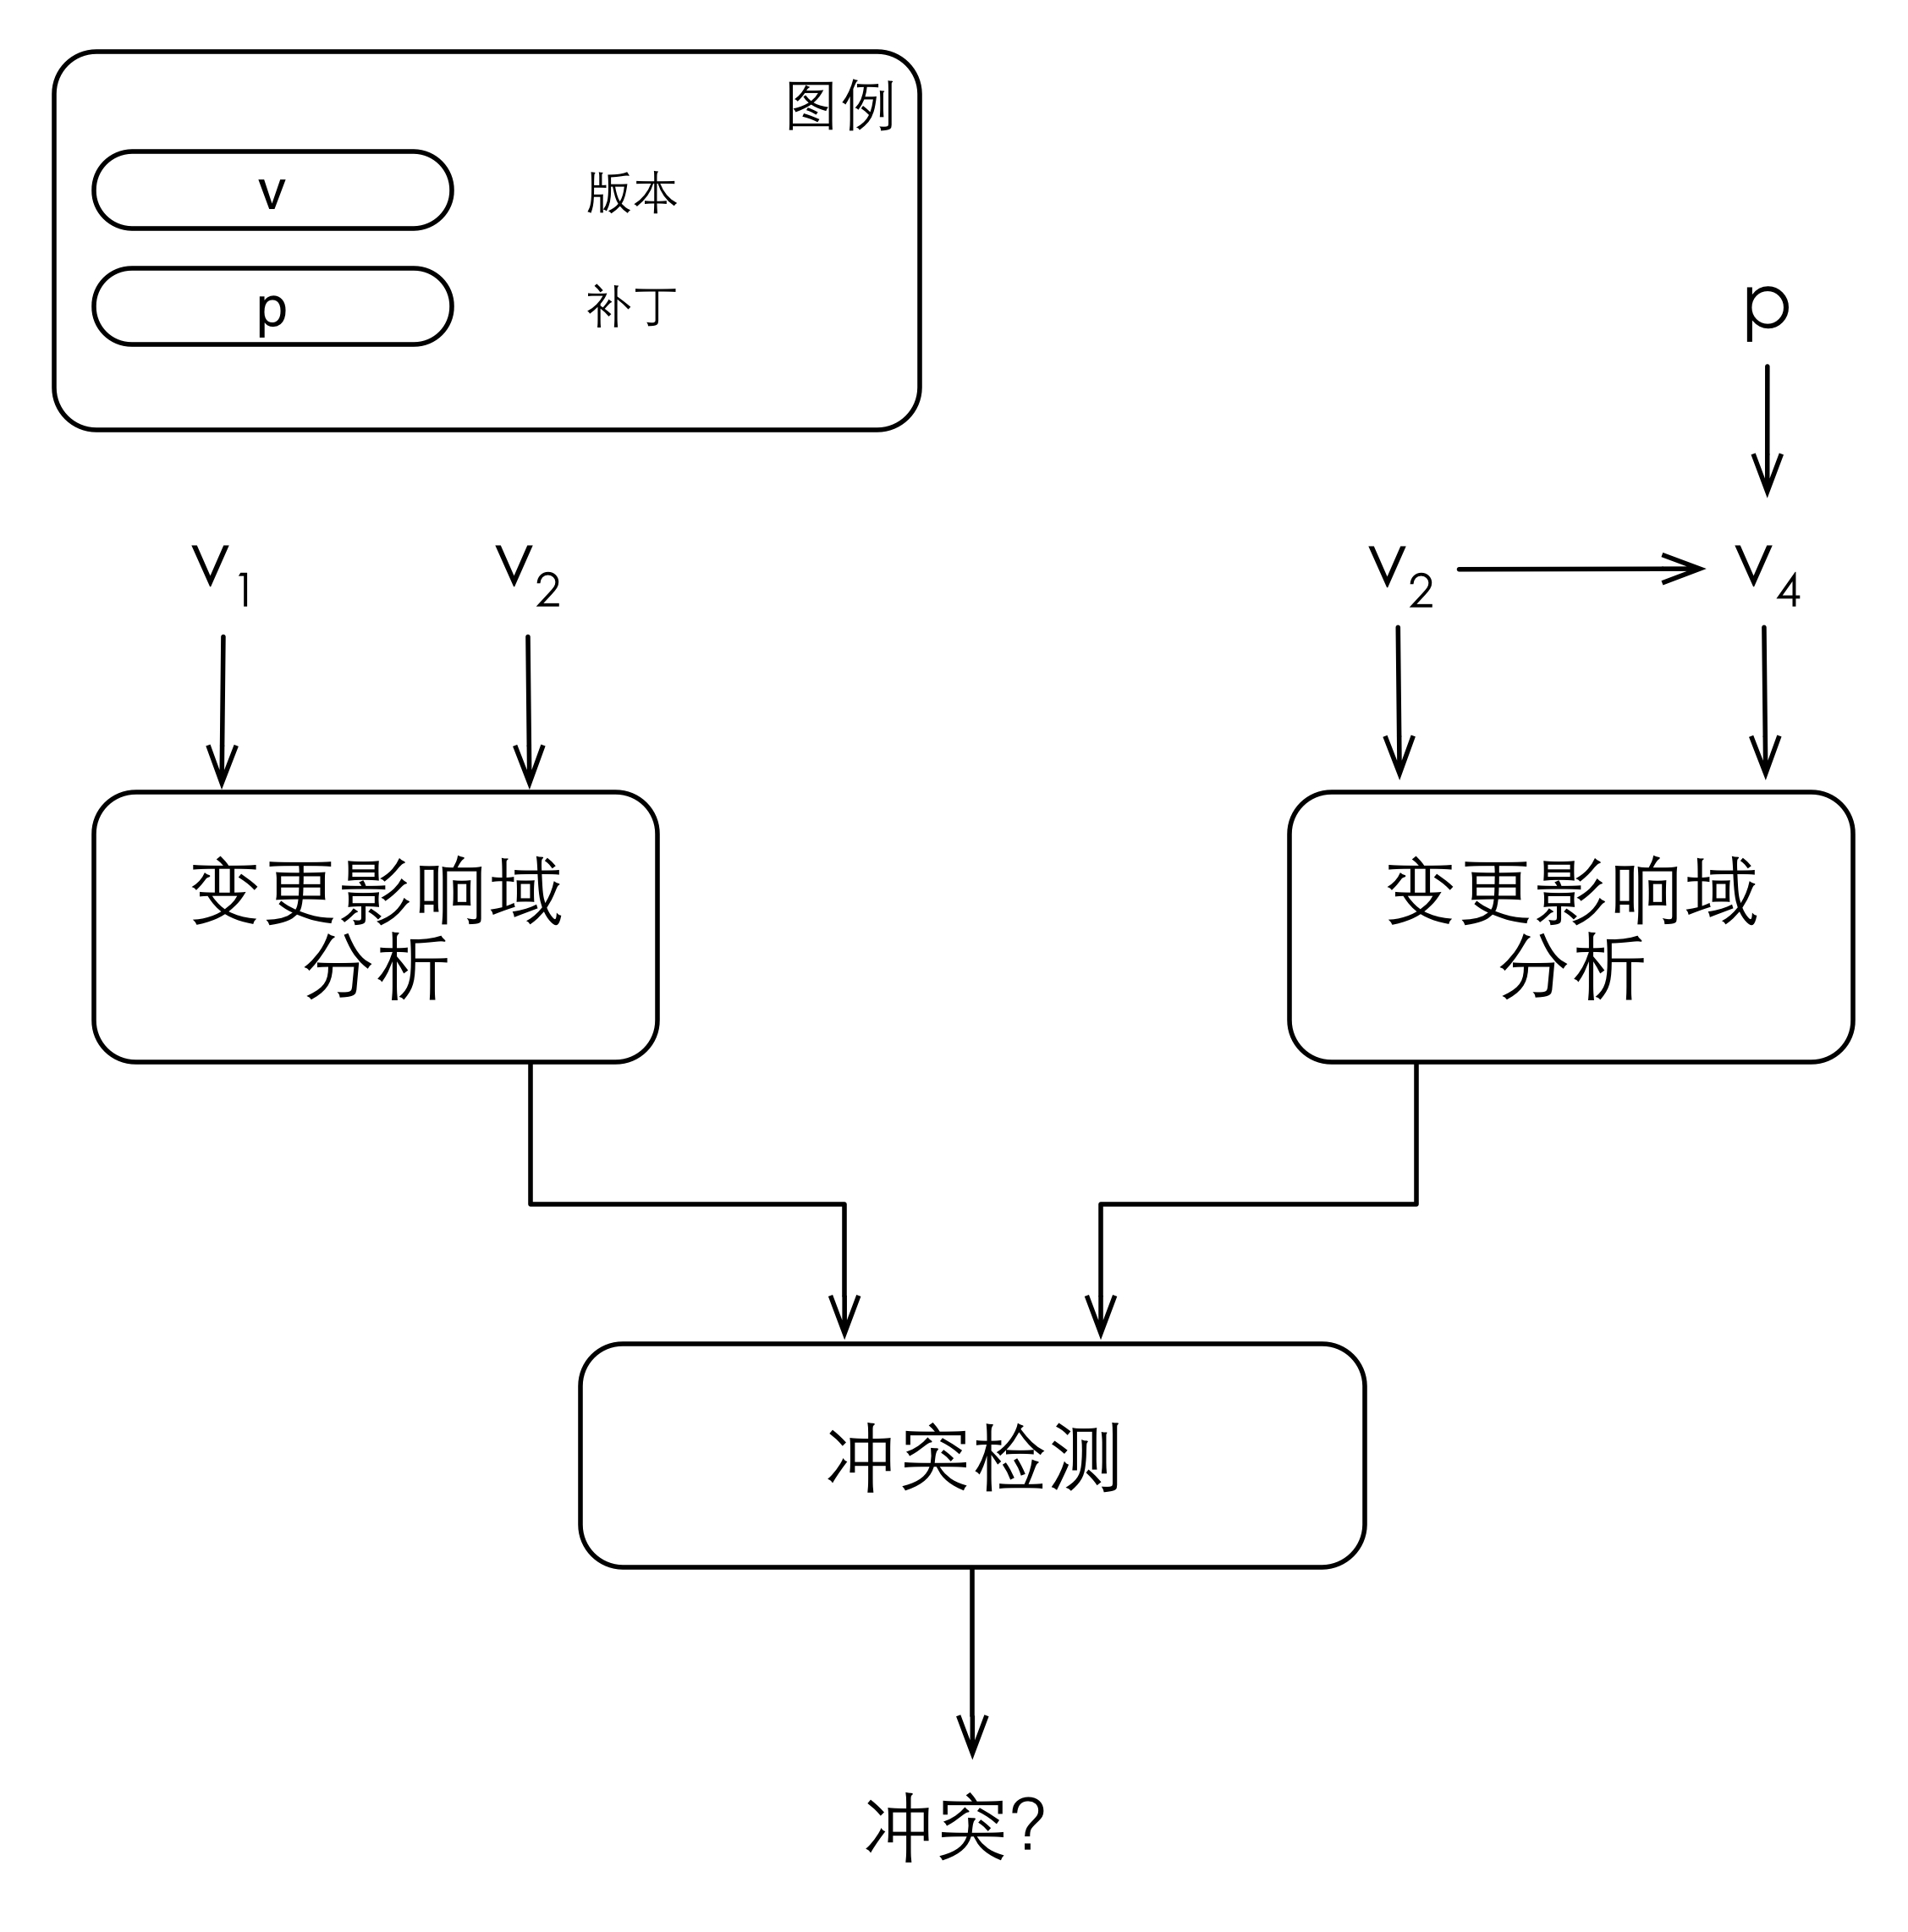
\includegraphics[height=.6\columnwidth]{chap03_all_now}
	\caption {检测方法}
	\label {all_flow}	
\end{figure}

该方法可以检测版本$v_1$到版本$v_2$的升级过程中所引入的变更是否会与补丁p在版本$v_2$中所引入的变更发生冲突。之所以选择以版本$v_2$作为基准来进行冲突检测,是由于在实际过程中,应用该检测方法之前还需要将补丁p应用至软件版本$v_2$,以完成补丁应用的过程。

本文采用了版本合并的方法来解决该过程中可能引入的语法错误,其流程简述如下:
\begin{enumerate}
	\item 将补丁p应用到版本$v_1$,获得旧版本应用补丁后的代码,其版本为$v_3$。
	\item 采用三路归并算法将版本$v_2$和$v_3$进行合并,获得新版本应用补丁后的代码,其版本为$v_4$。
	\item 解决版本合并中可能出现的冲突问题。
\end{enumerate}

最后所得到的$v_4$版本代码即为所需的在版本$v_2$上应用了补丁p中变更的新版本代码。

由于该合并过程较为简单,可以直接使用git等版本控制系统完成,以后的章节中将不再赘述,只在实验部分给出该过程相应的结果与分析。本文在以后的章节中将直接考虑对从版本$v_1$到$v_2$的升级过程中引入的变更与从版本$v_2$到$v_4$的升级过程中引入的变更进行冲突检测。

下面对该检测方法中所涉及到的过程进行概述。

首先,该检测方法中提出了一种软件变更影响域分析方法,该分析方法能够找到不同软件版本间的变更集合,并获取该变更集合所对应的语义影响域,即变更影响域,该变更影响域中包含了所有受到变更集合影响的程序语法结构。其中变更影响域分析过程可以分为两个子分析过程,先利用某种程序间语法差异性分析算法对输入的不同版本代码做差异性分析,得到以语法结构形式描述的变更集合,再使用某种变更语义影响分析算法去找到这些变更集合对软件代码的变更影响域。变更影响域分析的两个子过程可以自由替换为符合要求的相应算法实现,以提高检测方法的实用性。更具体的变更影响域分析过程和变更影响域等相关概念的定义可以参考章节\ref {chap_impact}中的叙述。

其次,该检测方法根据得到的不同变更影响域,使用软件变更冲突检测方法判定这些变更影响域之间是否存在着语义上的冲突。该检测方法主要实现了一种较为简单的自动冲突分析算法,通过计算变更影响域间的重叠来找到可能出现语义冲突的代码位置。更具体的冲突判定则有待进一步的人工分析来完成。该软件变更冲突检测方法的相关实现和定义可以参考章节\ref {chap_conflict}中的叙述。

最后得到的冲突检测结果即为所求。

本文根据此处提出的兼容性检测方法进行了相应的工具实现。按照兼容性检测方法的流程,该检测工具可以划分为两个模块,即影响域分析模块和冲突判定模块。

影响域分析模块主要实现了检测方法中的软件变更影响域分析方法。由于该方法由两个子分析过程组成,该模块在实现过程中同样划分为两个对应的子模块,即差异性分析子模块和影响分析子模块。由于这两个子分析过程已有相关的成熟算法实现,因此该模块采用了相关的分析工具来实现对应的算法,并按照本文的实际进行了一定的改进,因此该模块在实现过程中主要关注分析工具的整合和修改过程。

冲突判定模块则实现了检测方法中的软件变更冲突检测方法。该模块对软件变更冲突检测方法中提出的冲突检测算法进行了相应的实现,通过影响域分析模块给出的变更影响域来判断可能发生冲突的位置,即变更影响域的重叠位置。最后的冲突判定则由人工分析来完成。

%\begin{itemize}
%	\item 影响域分析模块:实现解决方案中的软件变更影响域分析过程。根据该过程的划分,该模块在实现过程中同样划分为两个子模块,即对应的差异性分析子模块和影响分析子模块。由于这两个子分析过程已有相关的成熟算法实现,因此实现过程中该模块采用了相关的分析工具来实现对应的算法,并按照本文的实际进行了一定的改进,即该模块在实现过程中主要关注分析工具的整合和修改过程。
%	\item 冲突判定模块:实现解决方案中的软件变更冲突检测方法。该模块对软件变更冲突检测方法中提出的检测算法进行了相应的实现,通过影响域分析模块给出的变更影响域来判断可能发生冲突的位置。
%\end{itemize}

以上模块的具体实现过程可以分别参考相关章节中的叙述。

\section{本章小结}
本章概括介绍了软件补丁兼容性问题和其检测方法。
章节~\ref{sec_problem} 中介绍了补丁兼容性问题。
章节\ref {sec_method}中对补丁兼容性检测方法和其工具实现进行了简要介绍。详细的介绍参见后续章节。


